
\Chapter{Results and discussion}{2D and 3D simulations and analytical approach.}

\section{2D results and discussion.}
\subsection{2D simulations}

\begin{figure}[htp]
\centering
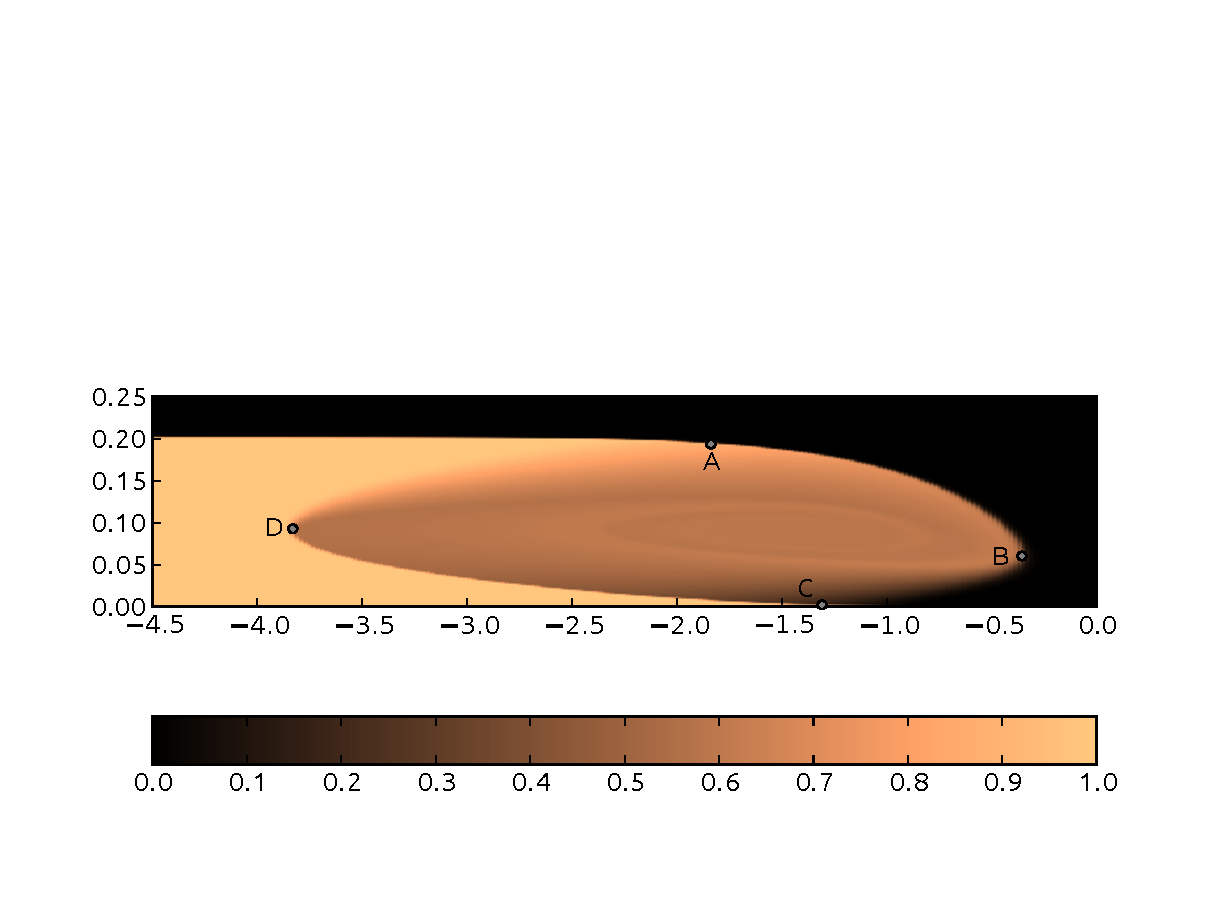
\includegraphics[scale=0.70]{vector/spiral_edit.pdf}
\caption{Steady state numerical solution for the 2D in the centre plane.}
\label{spiral}
\end{figure} 

The structure of the steady state can be very well explained qualitatively. Far from the head of the flow, the mixture is fully segregated. This is understandable: enough energy was given by the shearing process for the mixture to segregate during the flow's way down to the run-out pad. 

Closer from the head, a complex lens-shaped structure appear. It is delimited by two jumps in the concentration\footnote{See annex B for more details on jumps in segregation equations}, one from $A$ to $B$, the other from $C$ to $D$ (cf fig. \ref{spiral}). From $B$ to $C$ and from $D$ to $A$ the interface is dilute. It is what is called a rarefaction fan. Such fans are a common feature of conservation laws.

\begin{figure}[htp]
\centering
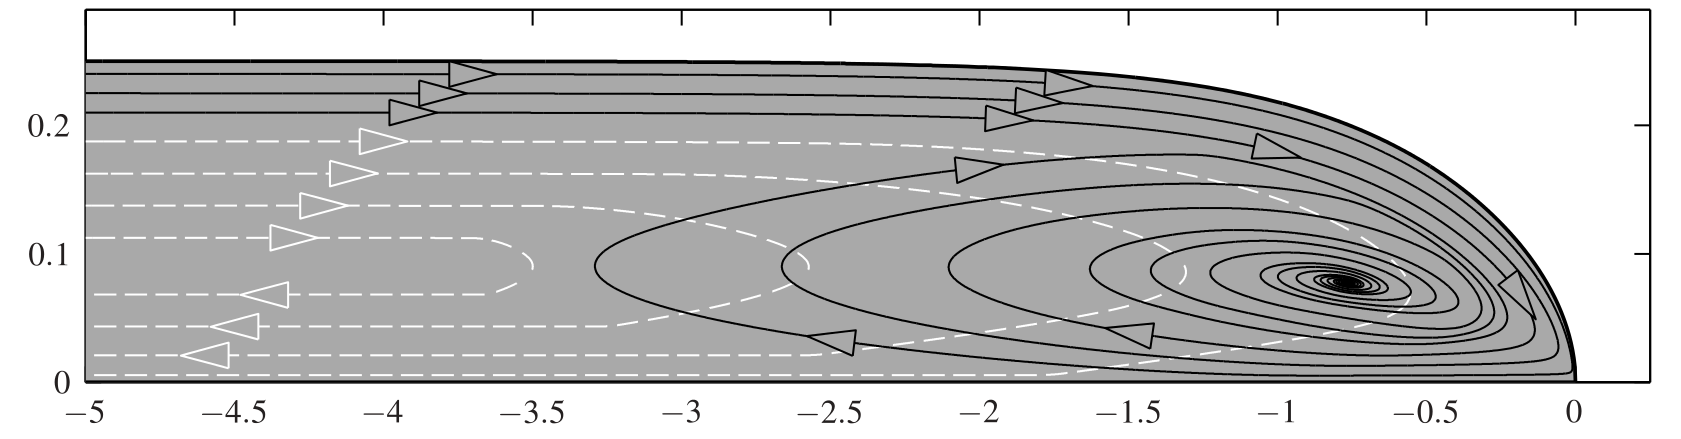
\includegraphics[scale=0.25]{images/pp.png}
\caption{Large particles paths (black lines) and small particles paths (white dotted lines) in the centre plane.}
\label{pp}
\end{figure} 

Inside the lens, we observe a mixture of small and large particles. 
If we compute the large particles trajectories (cf fig. \ref{pp}), we understand more clearly what is going on: large particles are going to the head faster than small ones. Therefore they are buried to the base of the flow, where they experience segregation. The combination of these two antagonist effects result in a spiral-like structure.

It is important to note, that if $\partial v / \partial y$ is zero, this spiral-like structure will \textit{not} appear. Cf for exemple \cite{2D}. In this article, a setup very similar to ours, but truly two dimensional is studied analytically. A similar lens-like structure is found to exist close to the head, and for the same reason. But here, because of the truly 2D nature of the problem, no spiral is observed.

The existence of a $\partial v / \partial y$ term implies that the 2D flow we analyse in the centre plane is compressible:
\begin{equation}
	\p{u}{x} + \p{w}{z} = - \p{v}{y} \neq 0
\end{equation} 
Qualitatively, this shows that some material from regions close to the centre plane is lost as it is advected to the sides of the flow. This advection occurs only close to the head, where the $\partial v / \partial y$ term is the highest in modulus.

\subsection{Analytical computations}

The geometrical \textit{method of characteristics} enables us to solve segregation equations in some particular situations. See appendix \ref{app:char} to see how it is done with a very simple example.
Following what we did in appendix \ref{app:char}  for the simplified segregation equation, we can do a change of coordinates to study the structure of our solution.
There is, however, a major difference between the two dimensional flow we studied in appendix \ref{app:char} and the one we study now.
In the simplified 2D case, the idea was to remap the $z$ axis: 
\begin{equation}
	z \leftarrow \psi(x,z)
\end{equation}
where $\psi$ is the stream function defined by 
\begin{equation}
	\begin{pmatrix}
	\p{\psi}{x}\\
	\p{\psi}{z} 
\end{pmatrix}
=
	\begin{pmatrix}
	-w\\
	u 
\end{pmatrix}
\end{equation}

Using the symmetry of second derivatives we see that the definition of $\psi$ implies
\begin{equation}
	\p{u}{x} + \p{w}{z} = 0
\end{equation}
which is the incompressibility condition for a 2D flow. Of course in 3D the incompressibility condition is
\begin{equation}
	\p{u}{x} + \p{v}{y} + \p{w}{z} = 0
\end{equation}
so we cannot define a stream function.
We need to use another function to remap the $z$ axis.

We notice that for a 2D stationary flow, the lines $\psi(x,z) = 0$ are the particle paths\footnote{Note that for a granular polydisperse flow, what we call "particle paths" are not the paths followed by actual particles. It is rather  the paths of hypothetical particles having their velocity equal to the bulk velocity.}.
So in the 3D case, rather than remapping the $z$ axis with a stream function, which is impossible, we will just say that our new $z$ coordinate is a -for now- unknown function $\z(x,z)$ which is constant along particle paths.

This property implies that
\begin{equation}
	\begin{pmatrix}
	\p{\z}{x}\\
	\p{\z}{z} 
\end{pmatrix}
\propto
	\begin{pmatrix}
	-w\\
	u 
\end{pmatrix}
\end{equation}
Let us call $\lam(x,z)$ the coefficient of proportionality. Of course if $\lam(x,z) = 1$ we have again
\begin{equation}
	\p{u}{x} + \p{w}{z} = 0
\end{equation}
so let us assume to begin with that $\lam$ is a function of $\zeta$ only : $\lam(x,z) = \hat{\lam}(\z)$

Expressing the velocity components in terms of derivatives of $\z$ in the 3D incompressibility equation yields
\begin{equation} \label{eq:lambda}
	- \underbrace{  \left( u \p{}{x} + w\p{}{z}\right) }_{\equiv D^\perp}  \log \lam(x,z) + \p{v}{y} = 0
\end{equation}
The operator $D^\perp$ appearing in the formula above plays a particular role.
Indeed if we call $\zperp$ a coordinate locally orthogonal to $\zeta$ we can easily see that
\begin{equation}
	D^\perp = u \p{}{x} + w\p{}{z} \propto \p{}{\zperp}
\end{equation}
so, if $\lam(x,z) = \hat{\lam}(\z)$ we have $D^\perp \hat \lam(\z) = 0$ and thus again
\begin{equation}
	\p{u}{x} + \p{w}{z} = 0
\end{equation}

Since making $\lam$ dependant or not on $\z$ does not have any impact on  eq. (\ref{eq:lambda}) I am going to assume for now on that $\lam$ is not a function of $\z$. In the system of coordinates $(x, \z)$ we can define $\lam$ as a function of $x$ only : $\lam = \lam(x)$.
In this system of coordinates, $D^\perp = u \p{}{x}$ and thus
\begin{equation}
	-u \tot{}{x} \log \lam + \p{v}{y} = 0
\end{equation}

Integrating this first order ordinary differential equation will give us $\lam(x)$ up to an arbitrary integration constant. Knowing $\lam(x)$, we can in turn know $\z(x,z)$, again up to an integration constant, using
\begin{equation}
	\begin{pmatrix}
	\p{\z}{x}\\
	\p{\z}{z} 
\end{pmatrix}
=
\lam(x)
	\begin{pmatrix}
	-w\\
	u 
\end{pmatrix}
\end{equation}
If we do that, we will have completely defined our change of coordinate $z \leftarrow \z$ and we will know it explicitly.
But is it useful to do this change of coordinates? Does it make it easier to find the structure of the steady-state solution as in the 2D case? We will see that it is indeed the case in the next section.

\subsection{Applying the change of coordinates to the segregation equation}

After the change of coordinates, the segregation equation becomes
\begin{equation}
	\p{\phi}{x} - \lam(x) \p{}{\z} \phi (1 - \phi) = 0
\end{equation}
This equation is exactly the one we have in the 2D case from appendix \ref{app:char}, after doing the change of coordinate $z \leftarrow \z(x,z)=\psi(x,z)$, except that in that case $\lam(x) = 1$.

Let $\z = Z(x)$ be a characteristic curve. And let us call $\Phi$ the (constant) value of  $\phi(x,\z)$ along the characteristic curve. We have
\begin{equation}
	\tot{Z}{x} = - \lam(x) ( 1 - 2 \Phi)
\end{equation}
Because $\lam$ depends on $x$ characteristics are not straight lines, contrary to what happens in the 2D case. 
To get around this problem, we can remap the $x$ axis : $x \leftarrow \x(x)$. 
In this new system of coordinates, characteristics will be straight lines if and only if
\begin{equation}
	\tot{\x}{x} = \lam(x)
\end{equation}
and the segregation equation becomes
\begin{equation}
	\p{\phi}{\x} - \p{}{\z} \phi (1 - \phi) = 0
\end{equation}

In this new coordinates system the jump condition\footnote{cf Appendix B} is of course simply the same as in the simplified case:
\begin{equation}
	\tot{\z}{\x} = \phi^+ + \phi^-  - 1
\end{equation}

The equation is the same as in 2D case, but we expect the solution to be different. Namely, to exhibit a "spiral" structure. 
Why is this spiral appearing? An hypothesis is that since the horizontal and vertical coordinates $\x$ and $\z$ can \textit{both} take the same value for different values of $x$ and $z$\footnote{in other words the inverse mapping $x = x(\x, \z)$ and $z = z(\x,\z)$ is multivalued}, the spatial domain in the remapped coordinates is a mosaic of smaller domains inside which $\x$ and $\z$ do not take the same value for different values of $x$ and $z$, each small domain forming a part of the spiral. \\

Sadly, tying to apply the method to the actual velocity field prescribed in the paper did not worked. 
Indeed, the velocity components have a rather complex analytical expression:

\begin{align}
	u(x, z) = 
	\left(\alpha -\frac{2 (\alpha -1) z}{H \sqrt{-\tanh \left(\frac{x}{W}\right)}}\right) \left(\frac{(2 n+1) U \sqrt{-\tanh \left(\frac{x}{W}\right)}}{(2 m+1) (2 m+2 n+1)}+\text{uF}\right)-\text{uF} \\
	w(x,z) = \frac{-z}{2 H W}
	\text{csch}\left(\frac{x}{W}\right) \text{sech}\left(\frac{x}{W}\right) \left(\frac{(2 n+1) U \left(2 (\alpha -1) z-\alpha  H \sqrt{-\tanh \left(\frac{x}{W}\right)}\right)}{(2 m+1) (2 m+2 n+1)}+\frac{(\alpha -1) \text{uF} z}{\sqrt{-\tanh \left(\frac{x}{W}\right)}}\right)
\end{align}

\subsection{Prescribing other velocity fields}

 \begin{figure}[htp]
\centering
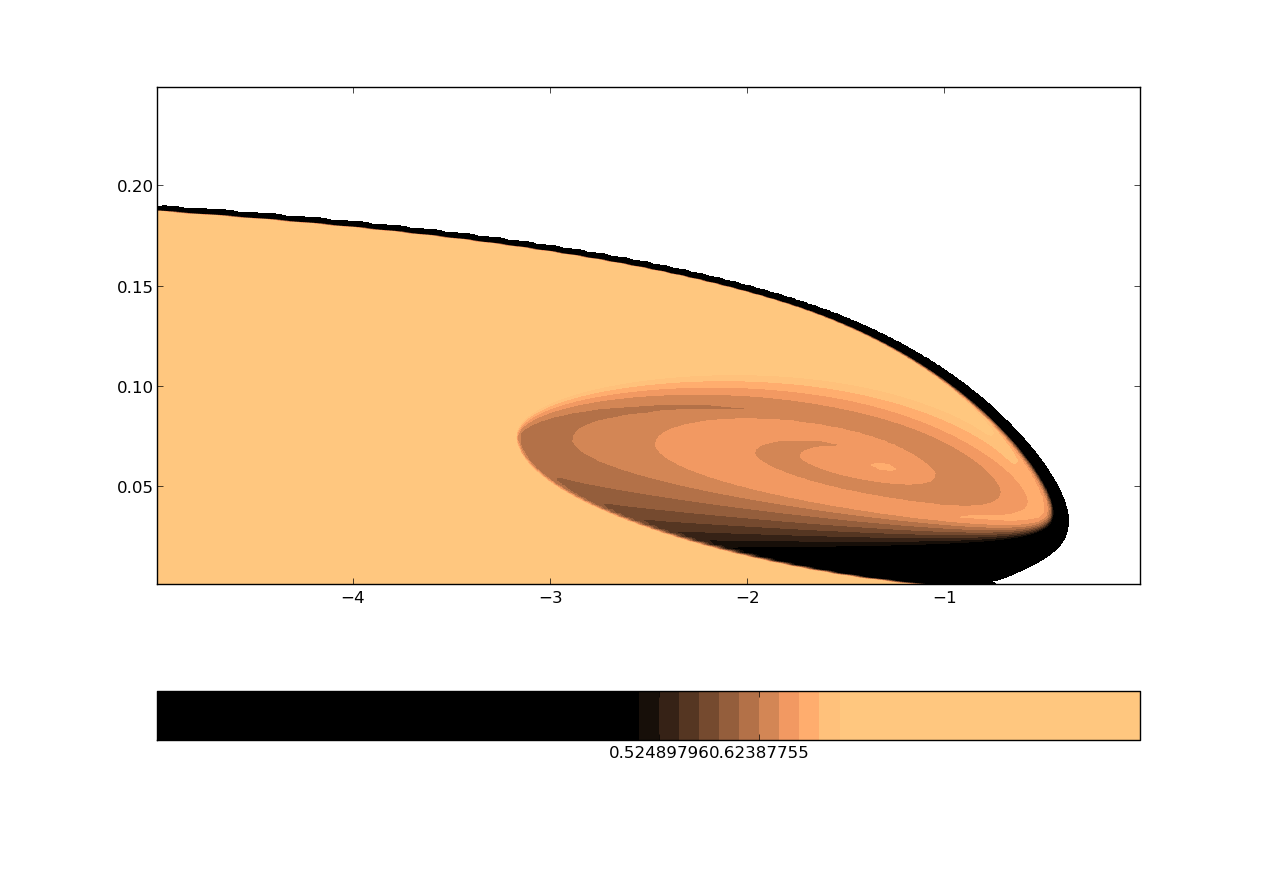
\includegraphics[scale=0.4]{images/rational_profile_spiral.png}
\caption{Steady-state numerical solution for the simplified velocity profile. The spiral structure is preserved.}
\label{rational}
\end{figure}


We were able to reproduce this spiral structures with a variety of different velocity fields. This is not surprising, if we have in mind that the origin of the spiral is 2D compressibility. 
There is therefore hope that we will eventually find a simpler velocity field, but for now, the simplest one we have been able to derive which still exhibit a spiral structure (fig \ref{rational}) is still too complex:
\[
 u =
 \left(
 \alpha 
 +\frac{2 (\alpha -1) z (W-x)}{H x}
 \right) 
 \left(
 u_F
 -\frac{(2 n+1) U x}{(2 m+1) (2 m+2 n+1) (W-x)}
 \right)-u_F
\]

\[
 w = 
 \frac{z \left(\frac{(2 n+1) U (x (\alpha  H-2 (\alpha -1) z)+2 (\alpha -1) W z)}{(2 m+1) (2 m+2 n+1)}-\frac{(\alpha -1) uF z (W-x)^2}{x}\right)}{H^2}
 \]

\section{3D generalisation}

The main goal of the internship was to produce a code capable of solving the full 3D problem as well as the 2D centre plane problem.
We chose to implement the Kurganov and Tadmor (KT) scheme \cite{KT}.
One of the advantages of this numerical scheme is that it is intrinsically dimension-independent. This allowed us to develop a code that can solve partial differential equations in any number of spatial dimensions. 

We first ran the code with the 2D problem in the centre plane, to make sure the results were in perfect agreement with the older code used in \cite{main}.

Then, we ran it for the full 3D setup. 
The result is of course impossible to plot, but we can visualize the restriction of the three dimensional concentration to a plan $y=\text{cst}$.
The results produced by these 3D simulations will be analysed in the future.

\begin{figure}[hbp]
\centering
\begin{subfigure}{.5\textwidth}
  \centering
  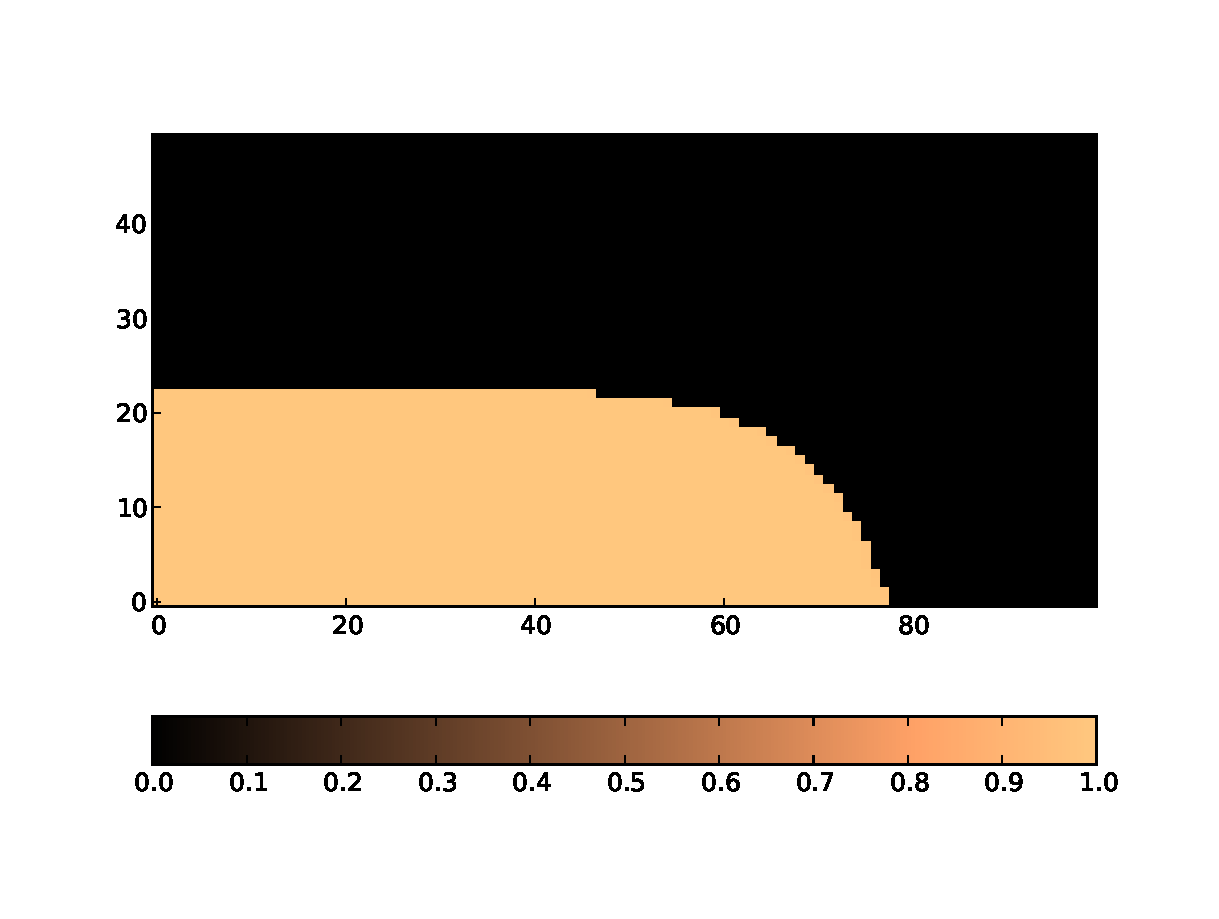
\includegraphics[width=.8\linewidth]{vector/3Dedge0}
  \caption{Initial concentration close to the aisles of the flow.}
  \label{}
\end{subfigure}%
\begin{subfigure}{.5\textwidth}
  \centering
  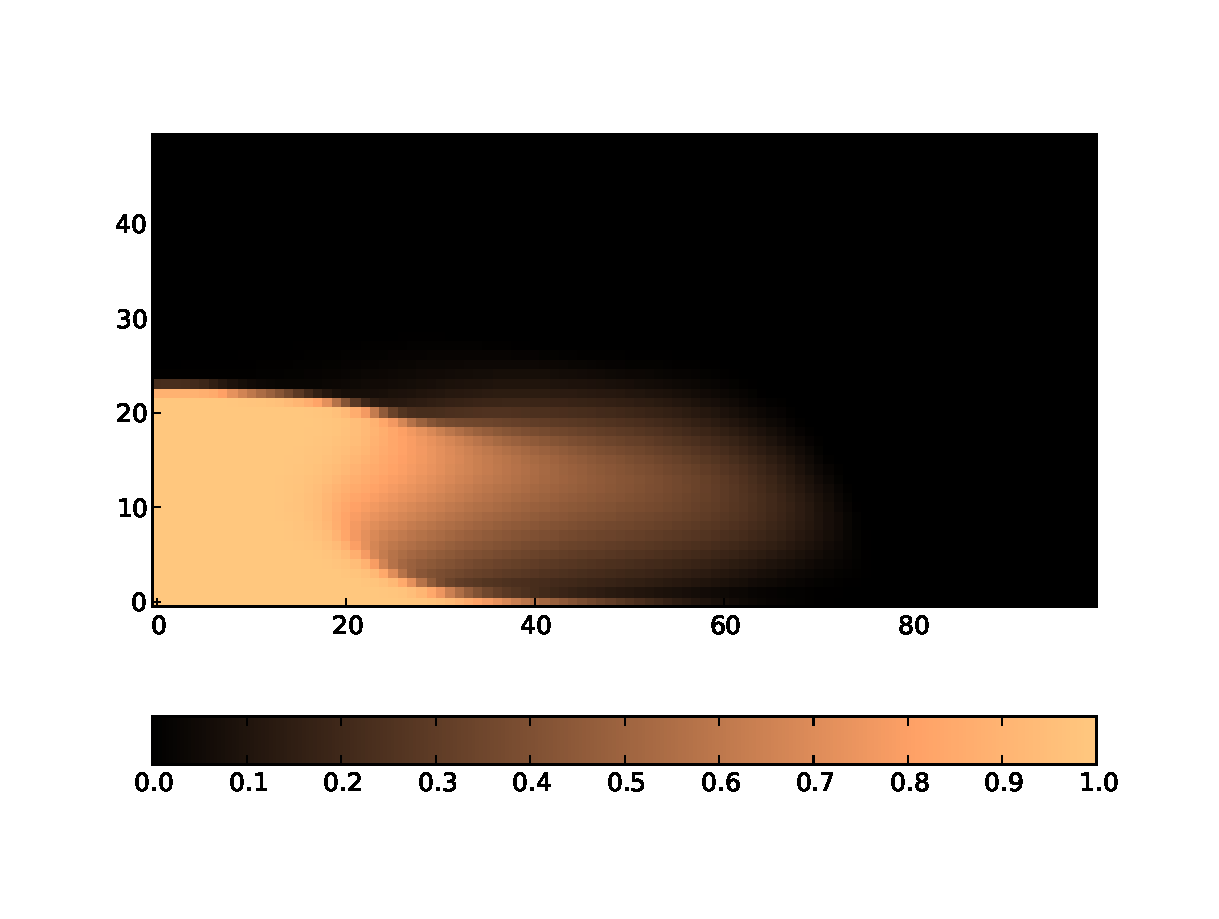
\includegraphics[width=.8\linewidth]{vector/3Dedge1}
  \caption{Concentration at the same location after some time.}
  \label{}
\end{subfigure}
\caption{The structure of the 3D flow is yet to be analysed.}
\label{fig:test}
\end{figure}
